% https://tex.stackexchange.com/questions/171982/how-to-make-table-floats-work-with-preview-standalone-environment/171983

\documentclass[%
    ,float=false % this is the new default and can be left away.
    ,preview=true
    ,class=scrartcl
%    ,fontsize=20pt
    ]{standalone}

\usepackage{amsmath}
\usepackage{tikz-dependency}
\DeclareMathOperator*{\argmax}{arg\,max}
\DeclareMathOperator*{\argmin}{arg\,min}
\DeclareMathOperator{\E}{\mathop{\mathbb{E}}}


\usepackage{xcite}
\externalcitedocument{pnas-word-order-si}



\usepackage{footnote}
\makesavenoteenv{tabular}
\makesavenoteenv{table}

\usepackage{siunitx}

\usepackage{longtable}


\usepackage[numbers]{natbib}


\usepackage{amssymb}% http://ctan.org/pkg/amssymb
\usepackage{pifont}% http://ctan.org/pkg/pifont
\newcommand{\cmark}{\ding{51}}%
\newcommand{\xmark}{\ding{55}}%

\usepackage[english]{babel}
\usepackage[utf8]{inputenc}
\usepackage{bm}
\usepackage{graphicx}
\usepackage{tikz}
\usepackage{xcolor}
\usepackage{url}
\usepackage{rotating}
\usepackage{multirow}
\usepackage{natbib}
\usepackage{arydshln}

\newcommand{\key}[1]{\textbf{#1}}



\renewcommand{\thefigure}{S\arabic{figure}}
\renewcommand{\thetable}{S\arabic{table}}
\renewcommand{\thesection}{S\arabic{section}}



\usepackage{mathtools}
\DeclarePairedDelimiter{\ceiling}{\lceil}{\rceil}


\begin{document}
\begin{tabular}{|l|l|l|ll|l|l|llllllllllllllllllllllllllll}
	\hline
&	Relation & Real &  Pred & Pars & Efficiency & Expected Prevalence  \\ \hline
% From Dryer	
\raisebox{.5pt}{\textcircled{\raisebox{-.9pt} {1}}}&	lifted\_case  &  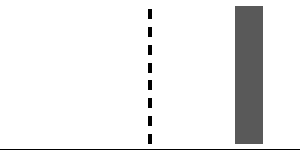
\includegraphics[width=0.06\textwidth]{../results/correlations/figures/posteriors/posterior_perRelation_Real_lifted_case.pdf}     &   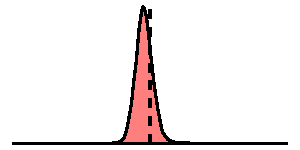
\includegraphics[width=0.06\textwidth]{../results/correlations/figures/posteriors/posterior_perRelation_Predictability_lifted_case.pdf}   &   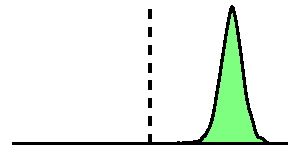
\includegraphics[width=0.06\textwidth]{../results/correlations/figures/posteriors/posterior_perRelation_Parseability_lifted_case.pdf}   &   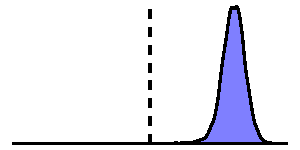
\includegraphics[width=0.06\textwidth]{../results/correlations/figures/posteriors/posterior_perRelation_Efficiency_lifted_case.pdf} & $> 50 \%$ \citep{dryer1992greenbergian}  \\
\raisebox{.5pt}{\textcircled{\raisebox{-.9pt} {2}}}&	lifted\_cop  &  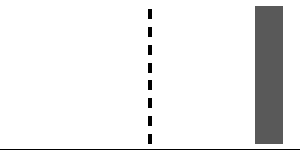
\includegraphics[width=0.06\textwidth]{../results/correlations/figures/posteriors/posterior_perRelation_Real_lifted_cop.pdf}      &   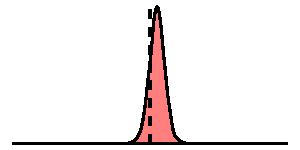
\includegraphics[width=0.06\textwidth]{../results/correlations/figures/posteriors/posterior_perRelation_Predictability_lifted_cop.pdf}   &   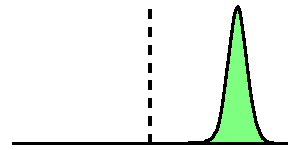
\includegraphics[width=0.06\textwidth]{../results/correlations/figures/posteriors/posterior_perRelation_Parseability_lifted_cop.pdf}   &   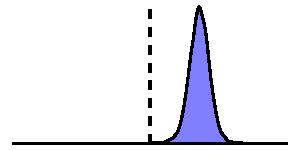
\includegraphics[width=0.06\textwidth]{../results/correlations/figures/posteriors/posterior_perRelation_Efficiency_lifted_cop.pdf} & $> 50 \%$ \citep{dryer1992greenbergian}  \\
\raisebox{.5pt}{\textcircled{\raisebox{-.9pt} {3}}}&	aux  &  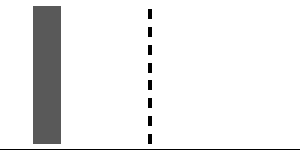
\includegraphics[width=0.06\textwidth]{../results/correlations/figures/posteriors/posterior_perRelation_Real_aux.pdf}      &   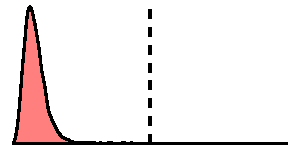
\includegraphics[width=0.06\textwidth]{../results/correlations/figures/posteriors/posterior_perRelation_Predictability_aux.pdf}   &   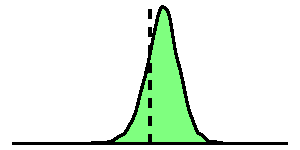
\includegraphics[width=0.06\textwidth]{../results/correlations/figures/posteriors/posterior_perRelation_Parseability_aux.pdf}   &   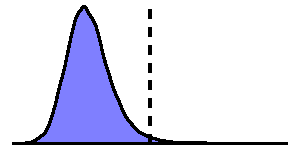
\includegraphics[width=0.06\textwidth]{../results/correlations/figures/posteriors/posterior_perRelation_Efficiency_aux.pdf}  & $>50\%$ \citep{dryer1992greenbergian} \\
\raisebox{.5pt}{\textcircled{\raisebox{-.9pt} {4}}}&	nmod  &  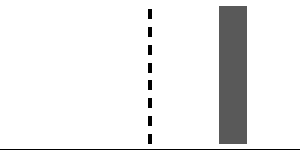
\includegraphics[width=0.06\textwidth]{../results/correlations/figures/posteriors/posterior_perRelation_Real_nmod.pdf}    &   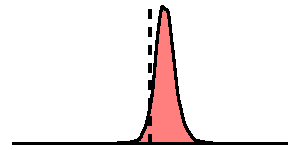
\includegraphics[width=0.06\textwidth]{../results/correlations/figures/posteriors/posterior_perRelation_Predictability_nmod.pdf}   &   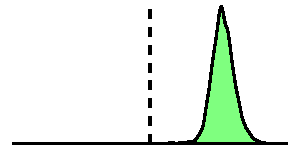
\includegraphics[width=0.06\textwidth]{../results/correlations/figures/posteriors/posterior_perRelation_Parseability_nmod.pdf}   &   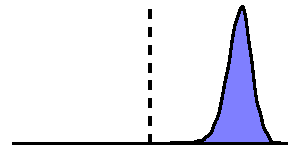
\includegraphics[width=0.06\textwidth]{../results/correlations/figures/posteriors/posterior_perRelation_Efficiency_nmod.pdf}  & $>50\%$ \citep{dryer1992greenbergian} \\
\raisebox{.5pt}{\textcircled{\raisebox{-.9pt} {5}}}&	acl  &  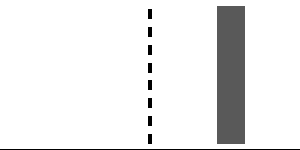
\includegraphics[width=0.06\textwidth]{../results/correlations/figures/posteriors/posterior_perRelation_Real_acl.pdf}    &   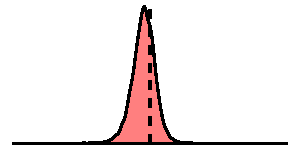
\includegraphics[width=0.06\textwidth]{../results/correlations/figures/posteriors/posterior_perRelation_Predictability_acl.pdf}  &   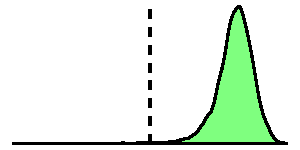
\includegraphics[width=0.06\textwidth]{../results/correlations/figures/posteriors/posterior_perRelation_Parseability_acl.pdf}  &  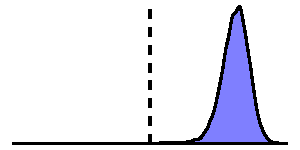
\includegraphics[width=0.06\textwidth]{../results/correlations/figures/posteriors/posterior_perRelation_Efficiency_acl.pdf}   & $>50\%$  \citep{dryer1992greenbergian} \\
\raisebox{.5pt}{\textcircled{\raisebox{-.9pt} {6}}}&	lifted\_mark  &  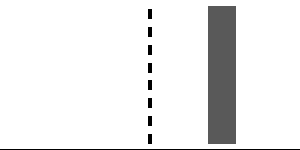
\includegraphics[width=0.06\textwidth]{../results/correlations/figures/posteriors/posterior_perRelation_Real_lifted_mark.pdf}      &   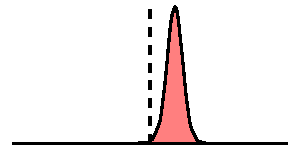
\includegraphics[width=0.06\textwidth]{../results/correlations/figures/posteriors/posterior_perRelation_Predictability_lifted_mark.pdf}   &   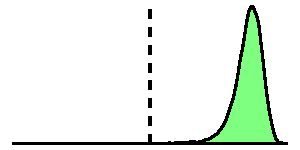
\includegraphics[width=0.06\textwidth]{../results/correlations/figures/posteriors/posterior_perRelation_Parseability_lifted_mark.pdf}   &   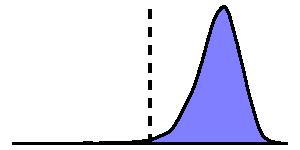
\includegraphics[width=0.06\textwidth]{../results/correlations/figures/posteriors/posterior_perRelation_Efficiency_lifted_mark.pdf} & $> 50 \%$ \citep{dryer1992greenbergian}  \\
\raisebox{.5pt}{\textcircled{\raisebox{-.9pt} {7}}}&	obl  &  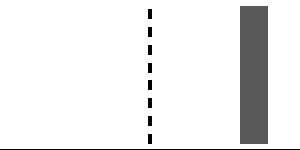
\includegraphics[width=0.06\textwidth]{../results/correlations/figures/posteriors/posterior_perRelation_Real_obl.pdf}      &   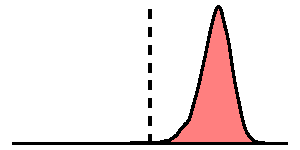
\includegraphics[width=0.06\textwidth]{../results/correlations/figures/posteriors/posterior_perRelation_Predictability_obl.pdf}   &   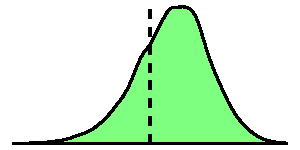
\includegraphics[width=0.06\textwidth]{../results/correlations/figures/posteriors/posterior_perRelation_Parseability_obl.pdf}   &   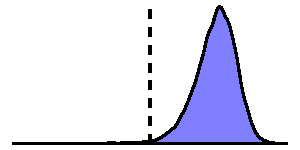
\includegraphics[width=0.06\textwidth]{../results/correlations/figures/posteriors/posterior_perRelation_Efficiency_obl.pdf}  & $>50\%$ \citep{dryer1992greenbergian} \\
\raisebox{.5pt}{\textcircled{\raisebox{-.9pt} {8}}}&	xcomp  &  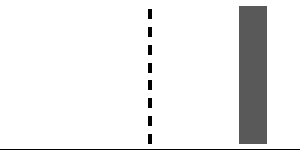
\includegraphics[width=0.06\textwidth]{../results/correlations/figures/posteriors/posterior_perRelation_Real_xcomp.pdf}     &   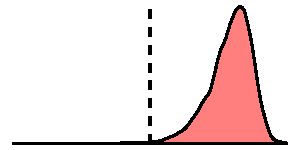
\includegraphics[width=0.06\textwidth]{../results/correlations/figures/posteriors/posterior_perRelation_Predictability_xcomp.pdf}   &   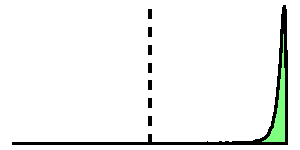
\includegraphics[width=0.06\textwidth]{../results/correlations/figures/posteriors/posterior_perRelation_Parseability_xcomp.pdf}   &   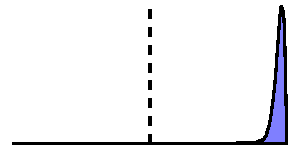
\includegraphics[width=0.06\textwidth]{../results/correlations/figures/posteriors/posterior_perRelation_Efficiency_xcomp.pdf}  & $>50\%$ \citep{dryer1992greenbergian} \\
%\hdashline

\hline
% Other universals, not in Dryer
&advcl  &  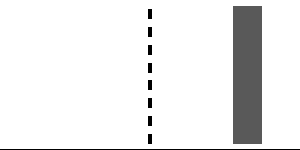
\includegraphics[width=0.06\textwidth]{../results/correlations/figures/posteriors/posterior_perRelation_Real_advcl.pdf}      &   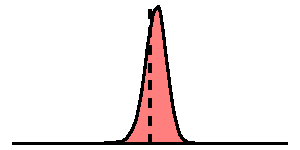
\includegraphics[width=0.06\textwidth]{../results/correlations/figures/posteriors/posterior_perRelation_Predictability_advcl.pdf}  &   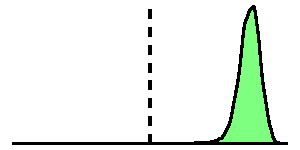
\includegraphics[width=0.06\textwidth]{../results/correlations/figures/posteriors/posterior_perRelation_Parseability_advcl.pdf}  &  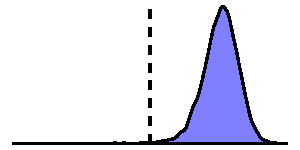
\includegraphics[width=0.06\textwidth]{../results/correlations/figures/posteriors/posterior_perRelation_Efficiency_advcl.pdf}   & $>50\%$ \citep{greenberg1963universals,diessel2001ordering} \\
&ccomp  &  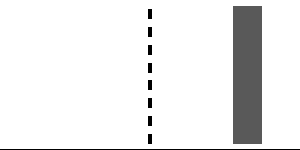
\includegraphics[width=0.06\textwidth]{../results/correlations/figures/posteriors/posterior_perRelation_Real_ccomp.pdf}      &   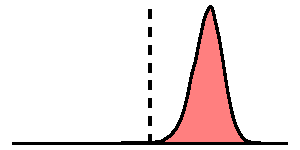
\includegraphics[width=0.06\textwidth]{../results/correlations/figures/posteriors/posterior_perRelation_Predictability_ccomp.pdf}  &   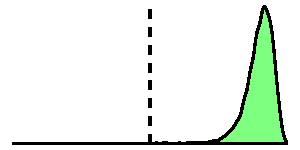
\includegraphics[width=0.06\textwidth]{../results/correlations/figures/posteriors/posterior_perRelation_Parseability_ccomp.pdf}  &  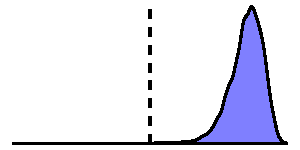
\includegraphics[width=0.06\textwidth]{../results/correlations/figures/posteriors/posterior_perRelation_Efficiency_ccomp.pdf}   & $>50\%$ (cf. \cite{dryer1980positional}) \\ % TODO According to Dryer 1980, there is a correlation
&csubj  &  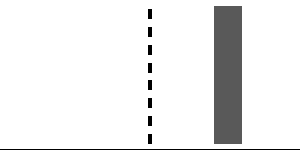
\includegraphics[width=0.06\textwidth]{../results/correlations/figures/posteriors/posterior_perRelation_Real_csubj.pdf}      &   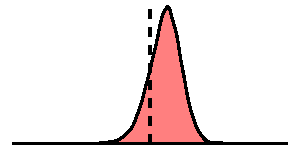
\includegraphics[width=0.06\textwidth]{../results/correlations/figures/posteriors/posterior_perRelation_Predictability_csubj.pdf}  &   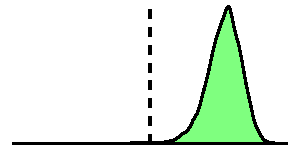
\includegraphics[width=0.06\textwidth]{../results/correlations/figures/posteriors/posterior_perRelation_Parseability_csubj.pdf}  &  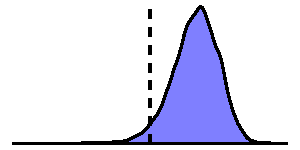
\includegraphics[width=0.06\textwidth]{../results/correlations/figures/posteriors/posterior_perRelation_Efficiency_csubj.pdf}   & $>50\%$ (cf. \cite{dryer1980positional}) \\% TODO According to Dryer 1980, there is a correlation
&nsubj  &  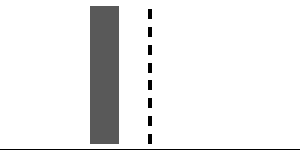
\includegraphics[width=0.06\textwidth]{../results/correlations/figures/posteriors/posterior_perRelation_Real_nsubj.pdf}      &   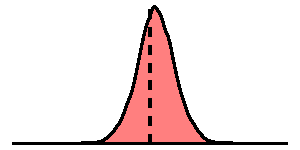
\includegraphics[width=0.06\textwidth]{../results/correlations/figures/posteriors/posterior_perRelation_Predictability_nsubj.pdf}   &   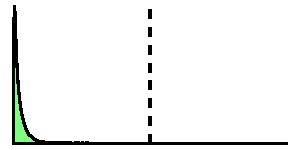
\includegraphics[width=0.06\textwidth]{../results/correlations/figures/posteriors/posterior_perRelation_Parseability_nsubj.pdf}   &   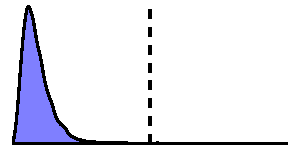
\includegraphics[width=0.06\textwidth]{../results/correlations/figures/posteriors/posterior_perRelation_Efficiency_nsubj.pdf}  & See Section S1 \\
&amod  &  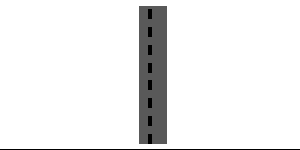
\includegraphics[width=0.06\textwidth]{../results/correlations/figures/posteriors/posterior_perRelation_Real_amod.pdf}      &   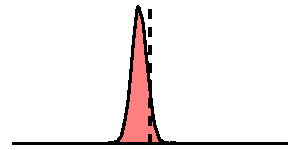
\includegraphics[width=0.06\textwidth]{../results/correlations/figures/posteriors/posterior_perRelation_Predictability_amod.pdf}  &   \includegraphics[width=0.06\textwidth]{../results/correlations/figures/posteriors/posterior_perRelation_Parseability_amod.pdf}  &  \includegraphics[width=0.06\textwidth]{../results/correlations/figures/posteriors/posterior_perRelation_Efficiency_amod.pdf}   &  $\approx 50\%$ \citep{dryer1992greenbergian} \\
&nummod  &  \includegraphics[width=0.06\textwidth]{../results/correlations/figures/posteriors/posterior_perRelation_Real_nummod.pdf}     &   \includegraphics[width=0.06\textwidth]{../results/correlations/figures/posteriors/posterior_perRelation_Predictability_nummod.pdf}  &   \includegraphics[width=0.06\textwidth]{../results/correlations/figures/posteriors/posterior_perRelation_Parseability_nummod.pdf}  &  \includegraphics[width=0.06\textwidth]{../results/correlations/figures/posteriors/posterior_perRelation_Efficiency_nummod.pdf}   &$\approx 50\%$ \citep[][89A, 83A]{wals} \\ 
 \hline
%comp. &
%\multirow{3}{*}{NP}&
%	AP &
\end{tabular}
\end{document}

